\chapter{Literature Review}

\graphicspath{{./Figures/Literature Review/}}


\section{Overview of Two-Wheeled Inverted Pendulum Robots (TWIPR)}
%vertical space
\vspace{2 cm}
%figure for Ascento robot
\begin {figure}[h]
\centering
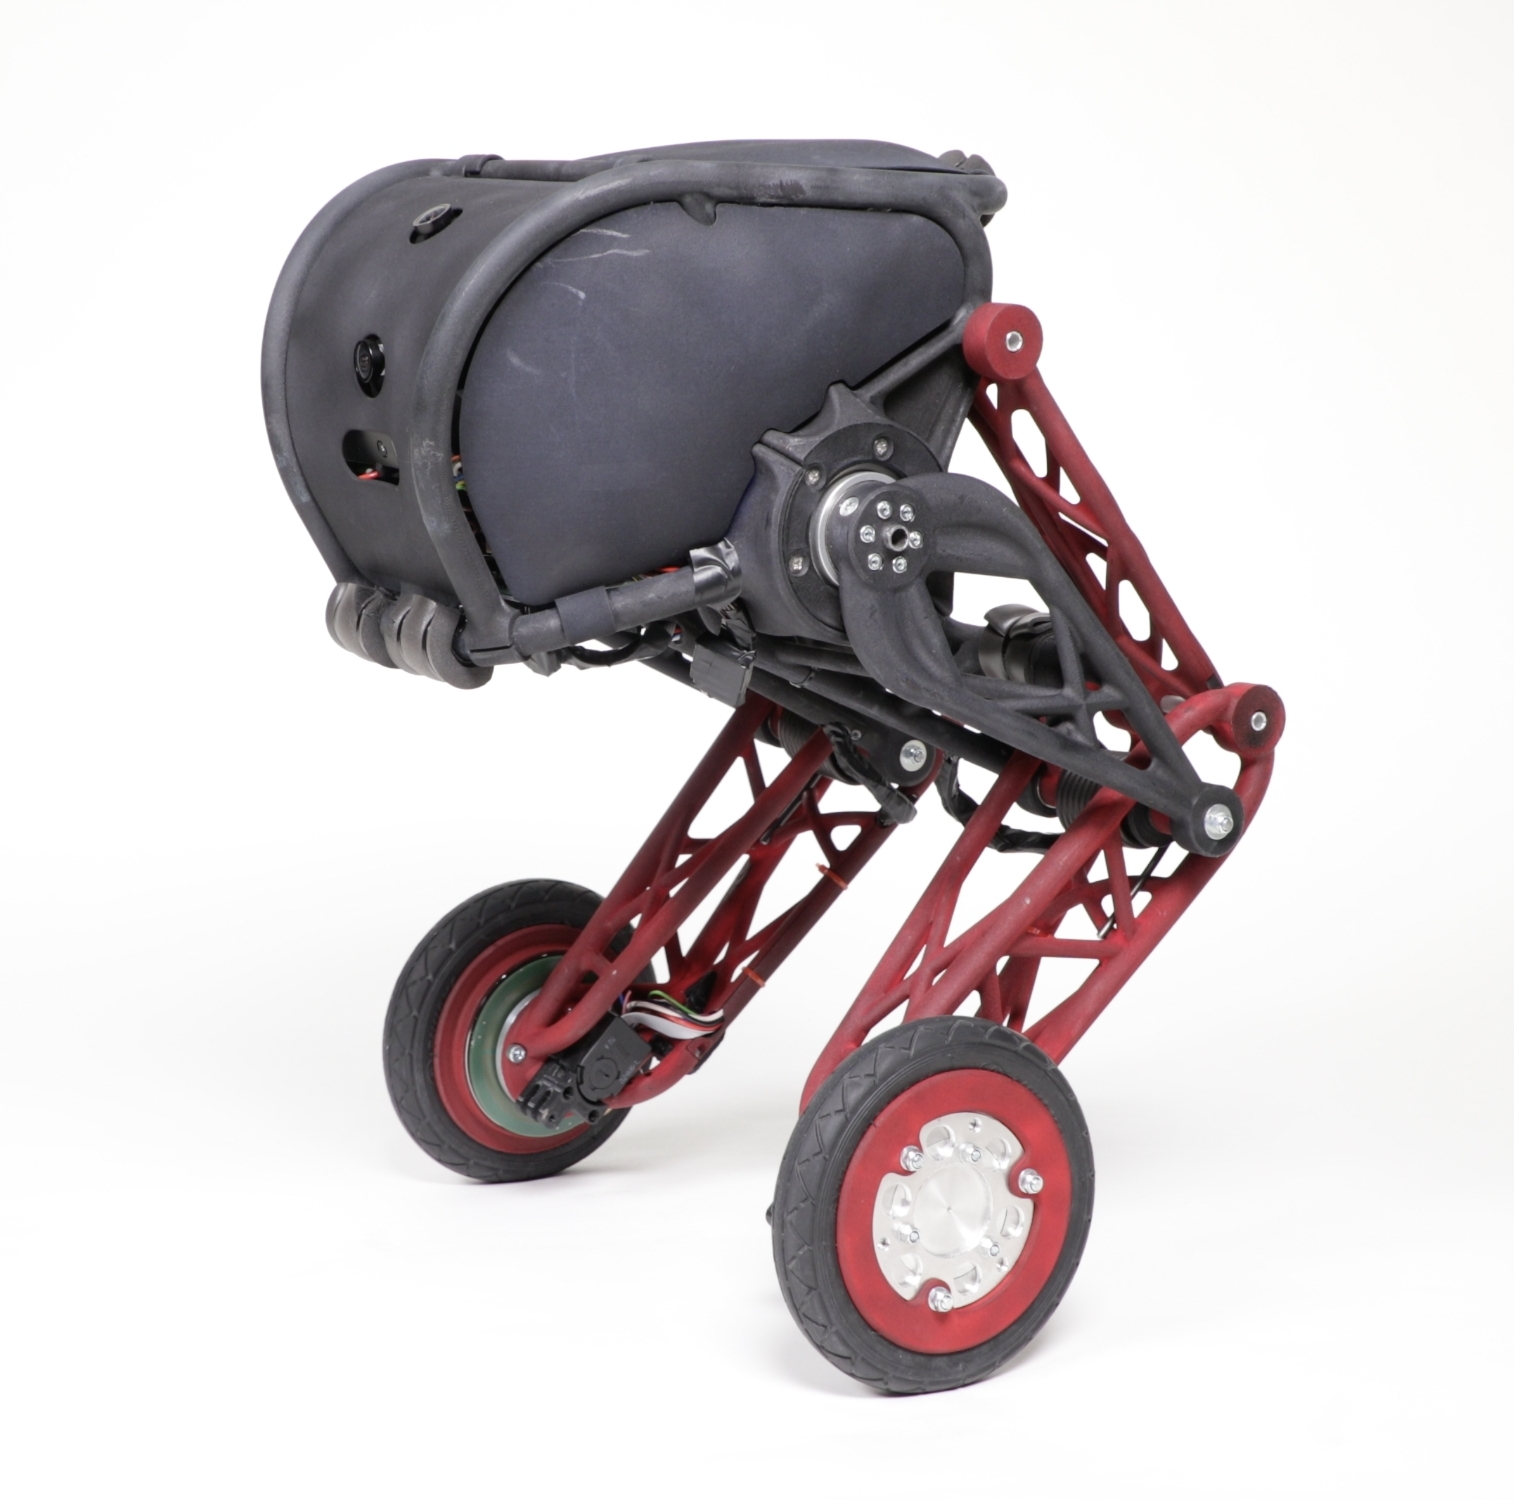
\includegraphics[width=0.5\textwidth]{Ascento robot}
\caption{Ascento Robot by ETH Zurich\cite{klemm2019ascento}}
\label{fig:Ascento robot}
\end {figure}

The Legged Two-Wheeled Inverted Pendulum Robot (LTWIPR) is a type of mobile robot that has two wheels and a body carried by two legs.
The robot acts as an inverted pendulum, with the wheels acting as the pivot point.
The robot is able to balance itself on the two wheels. The robot is able to move by tilting the body forward or backward, causing the wheels to rotate in the direction of the tilt. The robot is able to turn by moving the wheels in opposite directions. The robot is able to move in any direction by combining these movements. LTWIPRs are able to move in a variety of environments, including rough terrain and stairs. LTWIPRs are able to perform complex movements, such as jumping and climbing. LTWIPRs are able to interact with their environment, such as navigating around obstacles and diving under obstacles. LTWIPRs are able to perform tasks such as search and rescue, surveillance, and exploration.


\newpage
\section{Prior Works and Advances in Multi-Legged Robotic Systems}
%This section should provide a comprehensive review of existing literature relevant to your research topic. It should cover key theories, models, experiments, and findings in the field, particularly focusing on works that directly relate to your research question or hypothesis. This review not only shows your understanding of the field but also how your work fits into and contributes to the existing body of knowledge.
\subsection{Mechanical Design and Development of Wheeled Robots}
%three subfigures side by side for Honda's Asimo, Boston Dynamics' Atlas and sony QRIO
\begin {figure}[h]
\centering
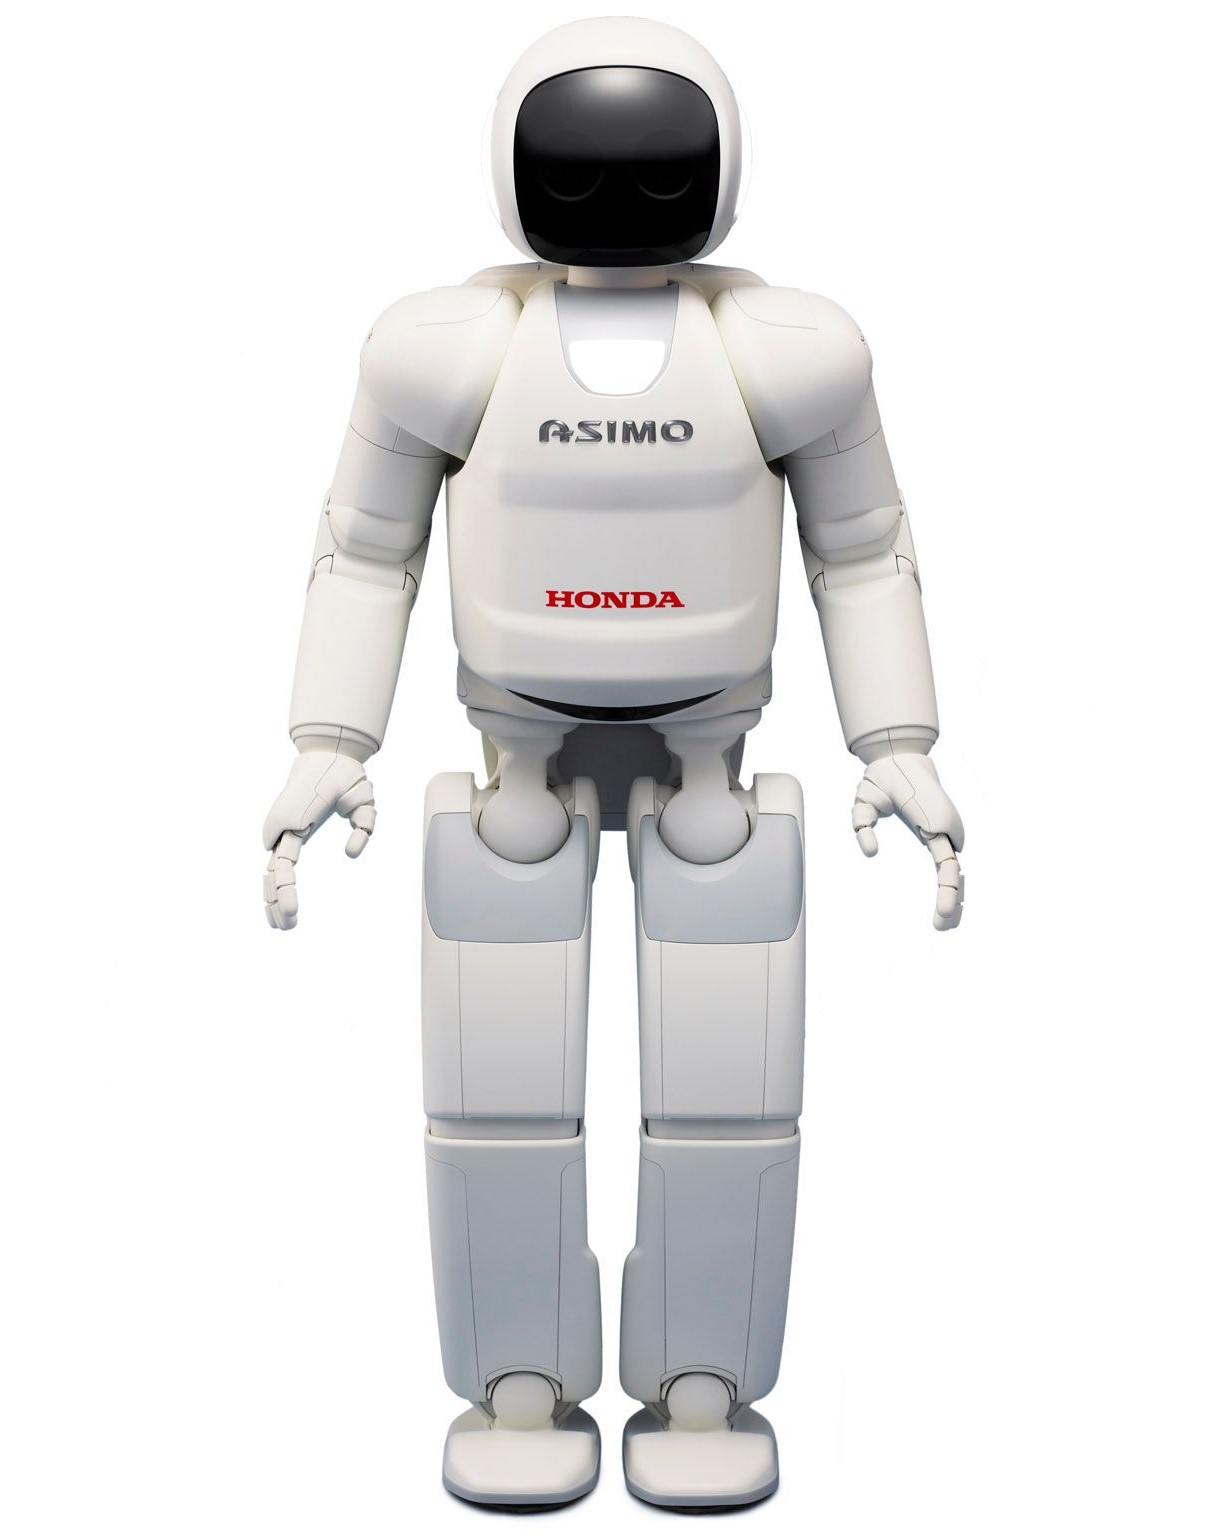
\includegraphics[width=0.3\textwidth]{Honda's Asimo}
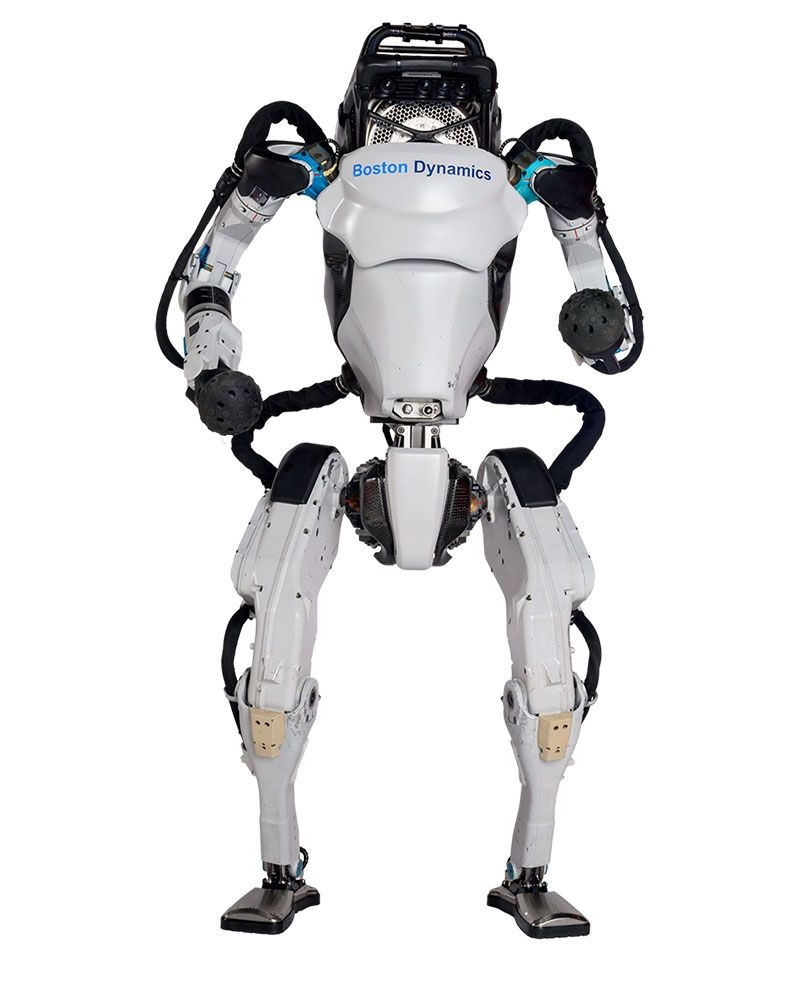
\includegraphics[width=0.3\textwidth]{Boston Dynamics' Atlas}
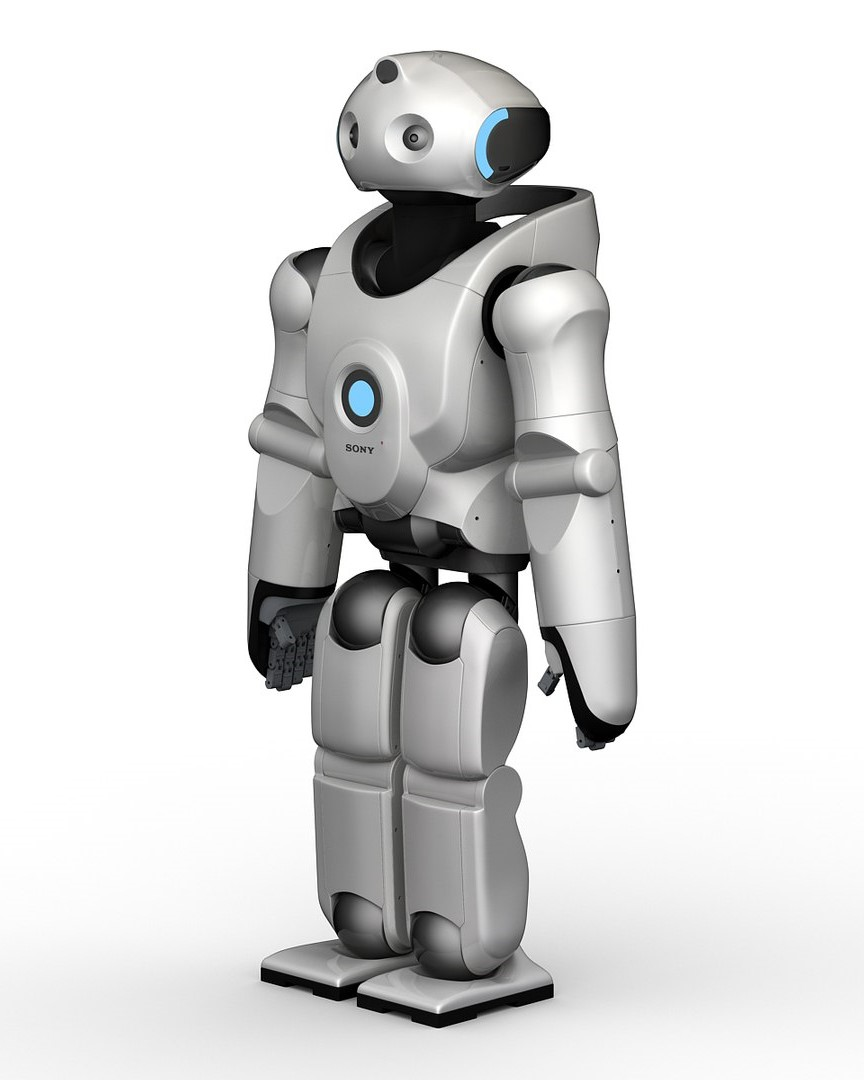
\includegraphics[width=0.3\textwidth]{sony QRIO}
\caption{Honda's Asimo, Boston Dynamics' Atlas and Sony QRIO\cite{asimo}\cite{atlas}\cite{qrio}}
\label{fig:Asimo, Atlas and QRIO}
\end {figure}


It is obvious that the mass distribution of the robot is a key factor in determining the robot's stability.
Various design considerations when designing a robot are important to consider such as the robot's size, degree of freedom, link design, and mass distribution \cite{nath2017design}.
Biped robots have many parameters that affect their locomotion, making it difficult to determine the right design parameters to achieve stable and reliable gaits.
The purpose of designing and assembling this biped robot is to advance research on humanoid robots and to offer a platform for studies on biped locomotion.
It is simple to change the structure to suit the researcher's interests and the type of testing that must be done.
As a result, the platform requires little upkeep.
With the help of sensors, electrical actuators, and mechanical connections, a biped robots with full functionality is put together to carry out a specific task.
An apparatus for processing (PU), primarily consisting of an embedded processor, which methodically regulates every part of the biped robot.
Several robots are built around these microcontrollers.
Because of the significant processing power that is contained on a single chip, programmers have a great deal of flexibility.
 \cite{madadi2007design}.
%figure for evoBOT-3
\begin {figure}[h]
\centering
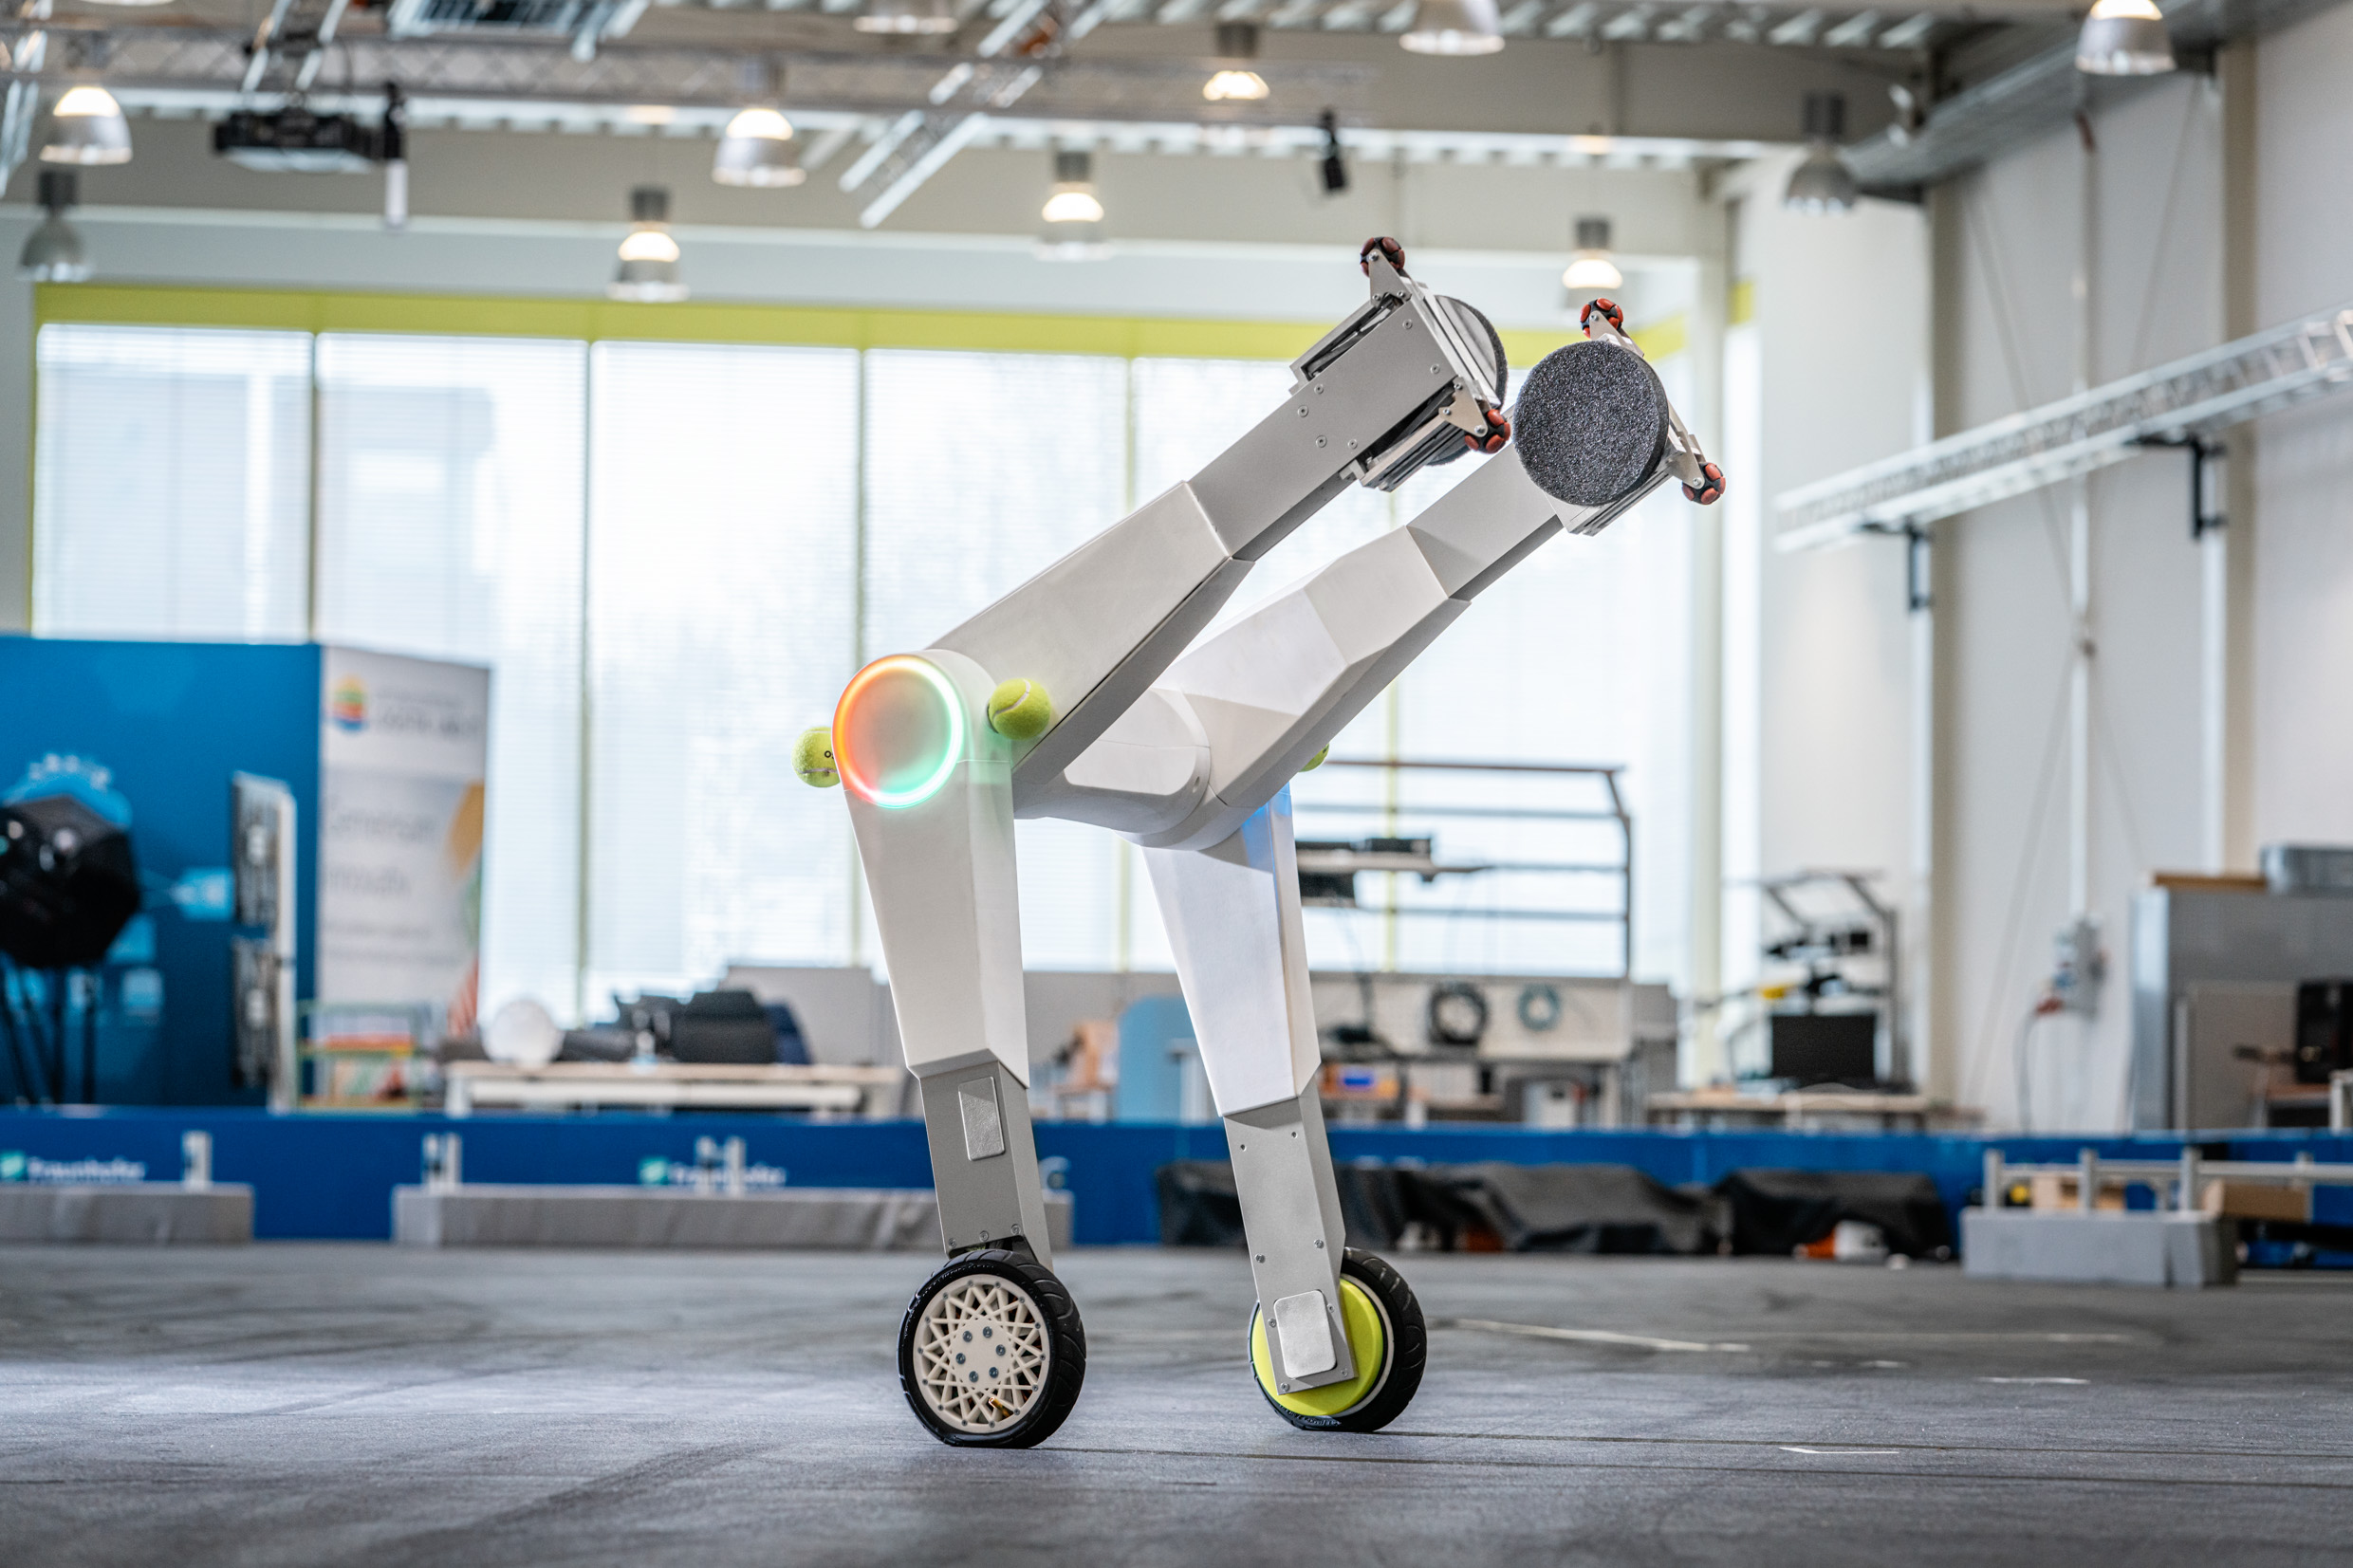
\includegraphics[width=0.5\textwidth]{evoBOT-3}
\caption{evoBOT-3\cite{klokowski2023evobot}}
\label{fig:evoBOT-3}
\end {figure}

The Legged Two-Wheeled Inverted Pendulum Robot (LTWIPR) such as the Ascento robot by ETH Zurich \cite{klemm2019ascento} and similar robots designs studied in \cite{guo2022design},\cite{zhang2022dynamic},\cite{cui2022modeling},\cite{hsu2022implementation} and \cite{xin2020online} demonstrate the different design approaches that can be used to design a LTWIPR. The wheel-leg hybrid design of the LTWIPR allows for the robot to have the advantages of both wheeled and legged robots.
another design differs, such as the evoBOT-3.
High levels of flexibility and agility define the evoBOT. This collaborative robot can be used in complex urban spaces, going beyond the traditional logistical context.
These extensions include load carriers and the passing and turning of objects.\cite{klokowski2023evobot}

\subsection{Dynamic Modeling of Wheeled Bipedal Robots}
The dynamic modeling of wheeled bipedal robots is a complex task that requires a thorough understanding of the robot's kinematics and dynamics.
 \cite{kim2015dynamic} outline the kinematics and dynamics of the Two-wheeled Inverted Pendulum Balancing
Mobile Robot where the kinematics constraints are derived and the dynamics are derived using the Lagrangian and Kane's methods. The equations of motions derived in this work can be considered as the base for the Legged Two-Wheeled Inverted Pendulum Robot (LTWIPR) since the Two-wheeled Inverted Pendulum Balancing Mobile Robot is a generalization of the LTWIPR.


\subsection{Control of Wheeled Bipedal Robots}
Different control strategies have been implemented on wheeled bipedal robots such as Fuzzy Logic, PID, LQR, MPC, and Reinforcement Learning.
The control strategies are chosen based on different factors such as the control objective, the complexity of the Robot's Dynamics and Requirements, The Robot's Operating Environment.

\subsection{Integration of Learning and Adaptive Control Mechanisms in Wheeled Bipedal Robots}

\subsection{Applications and Future Directions}
There are many applications for wheeled

